\begin{code}[hide]%
\>[0]\AgdaKeyword{module}\AgdaSpace{}%
\AgdaModule{vqupit.sections.two-routes}\AgdaSpace{}%
\AgdaKeyword{where}\<%
\\
%
\\[\AgdaEmptyExtraSkip]%
\>[0]\AgdaKeyword{open}\AgdaSpace{}%
\AgdaKeyword{import}\AgdaSpace{}%
\AgdaModule{Data.Nat}\AgdaSpace{}%
\AgdaKeyword{using}\AgdaSpace{}%
\AgdaSymbol{(}\AgdaDatatype{ℕ}\AgdaSymbol{)}\<%
\\
\>[0]\AgdaKeyword{open}\AgdaSpace{}%
\AgdaKeyword{import}\AgdaSpace{}%
\AgdaModule{Notations}\AgdaSpace{}%
\AgdaKeyword{using}\AgdaSpace{}%
\AgdaSymbol{(}\AgdaInductiveConstructor{₁₊}\AgdaSpace{}%
\AgdaSymbol{;}\AgdaSpace{}%
\AgdaInductiveConstructor{₂₊}\AgdaSymbol{)}\<%
\\
\>[0]\AgdaKeyword{open}\AgdaSpace{}%
\AgdaKeyword{import}\AgdaSpace{}%
\AgdaModule{Word.Base}\AgdaSpace{}%
\AgdaKeyword{using}\AgdaSpace{}%
\AgdaSymbol{(}\AgdaDatatype{Word}\AgdaSpace{}%
\AgdaSymbol{;}\AgdaSpace{}%
\AgdaFunction{WRel}\AgdaSpace{}%
\AgdaSymbol{;}\AgdaSpace{}%
\AgdaInductiveConstructor{ε}\AgdaSpace{}%
\AgdaSymbol{;}\AgdaSpace{}%
\AgdaOperator{\AgdaInductiveConstructor{\AgdaUnderscore{}•\AgdaUnderscore{}}}\AgdaSpace{}%
\AgdaSymbol{;}\AgdaSpace{}%
\AgdaOperator{\AgdaFunction{\AgdaUnderscore{}\textasciicircum{}\AgdaUnderscore{}}}\AgdaSymbol{)}\<%
\\
%
\\[\AgdaEmptyExtraSkip]%
\>[0]\AgdaKeyword{infixl}\AgdaSpace{}%
\AgdaNumber{9}\AgdaSpace{}%
\AgdaOperator{\AgdaPostulate{\AgdaUnderscore{}↑}}\AgdaSpace{}%
\AgdaOperator{\AgdaPostulate{\AgdaUnderscore{}↓}}\<%
\\
\>[0]\AgdaKeyword{infix}\AgdaSpace{}%
\AgdaNumber{4}\AgdaSpace{}%
\AgdaOperator{\AgdaDatatype{\AgdaUnderscore{}SRel,\AgdaUnderscore{}===\AgdaUnderscore{}}}\AgdaSpace{}%
\AgdaOperator{\AgdaPostulate{\AgdaUnderscore{}≈\AgdaUnderscore{}}}\<%
\\
\>[0]\AgdaKeyword{infix}\AgdaSpace{}%
\AgdaNumber{1}\AgdaSpace{}%
\AgdaOperator{\AgdaPostulate{begin\AgdaUnderscore{}}}\<%
\\
\>[0]\AgdaKeyword{infixr}\AgdaSpace{}%
\AgdaNumber{2}\AgdaSpace{}%
\AgdaOperator{\AgdaPostulate{\AgdaUnderscore{}≈⟨\AgdaUnderscore{}⟩\AgdaUnderscore{}}}\<%
\\
\>[0]\AgdaKeyword{infix}\AgdaSpace{}%
\AgdaNumber{3}\AgdaSpace{}%
\AgdaOperator{\AgdaPostulate{\AgdaUnderscore{}∎}}\<%
\\
\>[0]\AgdaKeyword{infixl}\AgdaSpace{}%
\AgdaNumber{3}\AgdaSpace{}%
\AgdaOperator{\AgdaPostulate{cleft\AgdaUnderscore{}}}\AgdaSpace{}%
\AgdaOperator{\AgdaPostulate{cright\AgdaUnderscore{}}}\<%
\\
%
\\[\AgdaEmptyExtraSkip]%
\>[0]\AgdaKeyword{private}\AgdaSpace{}%
\AgdaKeyword{variable}\<%
\\
\>[0][@{}l@{\AgdaIndent{0}}]%
\>[2]\AgdaGeneralizable{n}\AgdaSpace{}%
\AgdaSymbol{:}\AgdaSpace{}%
\AgdaDatatype{ℕ}\<%
\\
%
\\[\AgdaEmptyExtraSkip]%
\>[0]\AgdaKeyword{postulate}\<%
\\
\>[0][@{}l@{\AgdaIndent{0}}]%
\>[2]\AgdaPostulate{Gen}\AgdaSpace{}%
\AgdaSymbol{:}\AgdaSpace{}%
\AgdaDatatype{ℕ}\AgdaSpace{}%
\AgdaSymbol{→}\AgdaSpace{}%
\AgdaPrimitive{Set}\<%
\\
%
\>[2]\AgdaPostulate{H}\AgdaSpace{}%
\AgdaPostulate{S}\AgdaSpace{}%
\AgdaPostulate{CZ}\AgdaSpace{}%
\AgdaSymbol{:}\AgdaSpace{}%
\AgdaSymbol{∀}\AgdaSpace{}%
\AgdaSymbol{\{}\AgdaBound{n}\AgdaSymbol{\}}\AgdaSpace{}%
\AgdaSymbol{→}\AgdaSpace{}%
\AgdaDatatype{Word}\AgdaSpace{}%
\AgdaSymbol{(}\AgdaPostulate{Gen}\AgdaSpace{}%
\AgdaBound{n}\AgdaSymbol{)}\<%
\\
%
\>[2]\AgdaOperator{\AgdaPostulate{\AgdaUnderscore{}↑}}\AgdaSpace{}%
\AgdaOperator{\AgdaPostulate{\AgdaUnderscore{}↓}}\AgdaSpace{}%
\AgdaSymbol{:}\AgdaSpace{}%
\AgdaSymbol{∀}\AgdaSpace{}%
\AgdaSymbol{\{}\AgdaBound{n}\AgdaSymbol{\}}\AgdaSpace{}%
\AgdaSymbol{→}\AgdaSpace{}%
\AgdaDatatype{Word}\AgdaSpace{}%
\AgdaSymbol{(}\AgdaPostulate{Gen}\AgdaSpace{}%
\AgdaBound{n}\AgdaSymbol{)}\AgdaSpace{}%
\AgdaSymbol{→}\AgdaSpace{}%
\AgdaDatatype{Word}\AgdaSpace{}%
\AgdaSymbol{(}\AgdaPostulate{Gen}\AgdaSpace{}%
\AgdaBound{n}\AgdaSymbol{)}\<%
\\
%
\>[2]\AgdaOperator{\AgdaPostulate{\AgdaUnderscore{}≈\AgdaUnderscore{}}}\AgdaSpace{}%
\AgdaSymbol{:}\AgdaSpace{}%
\AgdaSymbol{∀}\AgdaSpace{}%
\AgdaSymbol{\{}\AgdaBound{n}\AgdaSymbol{\}}\AgdaSpace{}%
\AgdaSymbol{→}\AgdaSpace{}%
\AgdaDatatype{Word}\AgdaSpace{}%
\AgdaSymbol{(}\AgdaPostulate{Gen}\AgdaSpace{}%
\AgdaBound{n}\AgdaSymbol{)}\AgdaSpace{}%
\AgdaSymbol{→}\AgdaSpace{}%
\AgdaDatatype{Word}\AgdaSpace{}%
\AgdaSymbol{(}\AgdaPostulate{Gen}\AgdaSpace{}%
\AgdaBound{n}\AgdaSymbol{)}\AgdaSpace{}%
\AgdaSymbol{→}\AgdaSpace{}%
\AgdaPrimitive{Set}\<%
\\
%
\>[2]\AgdaOperator{\AgdaPostulate{begin\AgdaUnderscore{}}}\AgdaSpace{}%
\AgdaSymbol{:}\AgdaSpace{}%
\AgdaSymbol{∀}\AgdaSpace{}%
\AgdaSymbol{\{}\AgdaBound{n}\AgdaSymbol{\}}\AgdaSpace{}%
\AgdaSymbol{\{}\AgdaBound{w}\AgdaSpace{}%
\AgdaBound{v}\AgdaSpace{}%
\AgdaSymbol{:}\AgdaSpace{}%
\AgdaDatatype{Word}\AgdaSpace{}%
\AgdaSymbol{(}\AgdaPostulate{Gen}\AgdaSpace{}%
\AgdaBound{n}\AgdaSymbol{)\}}\AgdaSpace{}%
\AgdaSymbol{→}\AgdaSpace{}%
\AgdaBound{w}\AgdaSpace{}%
\AgdaOperator{\AgdaPostulate{≈}}\AgdaSpace{}%
\AgdaBound{v}\AgdaSpace{}%
\AgdaSymbol{→}\AgdaSpace{}%
\AgdaBound{w}\AgdaSpace{}%
\AgdaOperator{\AgdaPostulate{≈}}\AgdaSpace{}%
\AgdaBound{v}\<%
\\
%
\>[2]\AgdaOperator{\AgdaPostulate{\AgdaUnderscore{}≈⟨\AgdaUnderscore{}⟩\AgdaUnderscore{}}}\AgdaSpace{}%
\AgdaSymbol{:}\AgdaSpace{}%
\AgdaSymbol{∀}\AgdaSpace{}%
\AgdaSymbol{\{}\AgdaBound{n}\AgdaSymbol{\}}\AgdaSpace{}%
\AgdaSymbol{(}\AgdaBound{w}\AgdaSpace{}%
\AgdaSymbol{:}\AgdaSpace{}%
\AgdaDatatype{Word}\AgdaSpace{}%
\AgdaSymbol{(}\AgdaPostulate{Gen}\AgdaSpace{}%
\AgdaBound{n}\AgdaSymbol{))}\AgdaSpace{}%
\AgdaSymbol{\{}\AgdaBound{v}\AgdaSpace{}%
\AgdaBound{u}\AgdaSymbol{\}}\AgdaSpace{}%
\AgdaSymbol{→}\AgdaSpace{}%
\AgdaBound{w}\AgdaSpace{}%
\AgdaOperator{\AgdaPostulate{≈}}\AgdaSpace{}%
\AgdaBound{v}\AgdaSpace{}%
\AgdaSymbol{→}\AgdaSpace{}%
\AgdaBound{v}\AgdaSpace{}%
\AgdaOperator{\AgdaPostulate{≈}}\AgdaSpace{}%
\AgdaBound{u}\AgdaSpace{}%
\AgdaSymbol{→}\AgdaSpace{}%
\AgdaBound{w}\AgdaSpace{}%
\AgdaOperator{\AgdaPostulate{≈}}\AgdaSpace{}%
\AgdaBound{u}\<%
\\
%
\>[2]\AgdaOperator{\AgdaPostulate{\AgdaUnderscore{}∎}}\AgdaSpace{}%
\AgdaSymbol{:}\AgdaSpace{}%
\AgdaSymbol{∀}\AgdaSpace{}%
\AgdaSymbol{\{}\AgdaBound{n}\AgdaSymbol{\}}\AgdaSpace{}%
\AgdaSymbol{(}\AgdaBound{w}\AgdaSpace{}%
\AgdaSymbol{:}\AgdaSpace{}%
\AgdaDatatype{Word}\AgdaSpace{}%
\AgdaSymbol{(}\AgdaPostulate{Gen}\AgdaSpace{}%
\AgdaBound{n}\AgdaSymbol{))}\AgdaSpace{}%
\AgdaSymbol{→}\AgdaSpace{}%
\AgdaBound{w}\AgdaSpace{}%
\AgdaOperator{\AgdaPostulate{≈}}\AgdaSpace{}%
\AgdaBound{w}\<%
\\
%
\>[2]\AgdaPostulate{sym}\AgdaSpace{}%
\AgdaPostulate{assoc}\AgdaSpace{}%
\AgdaPostulate{right-unit}\AgdaSpace{}%
\AgdaOperator{\AgdaPostulate{cleft\AgdaUnderscore{}}}\AgdaSpace{}%
\AgdaOperator{\AgdaPostulate{cright\AgdaUnderscore{}}}\AgdaSpace{}%
\AgdaPostulate{axiom}\AgdaSpace{}%
\AgdaSymbol{:}\AgdaSpace{}%
\AgdaSymbol{∀}\AgdaSpace{}%
\AgdaSymbol{\{}\AgdaBound{ℓ}\AgdaSymbol{\}}\AgdaSpace{}%
\AgdaSymbol{\{}\AgdaBound{A}\AgdaSpace{}%
\AgdaSymbol{:}\AgdaSpace{}%
\AgdaPrimitive{Set}\AgdaSpace{}%
\AgdaBound{ℓ}\AgdaSymbol{\}}\AgdaSpace{}%
\AgdaSymbol{→}\AgdaSpace{}%
\AgdaBound{A}\<%
\end{code}
\section{Qupit Clifford Operators and Two Routes to Completeness}\label{sec:two-routes}

This section recalls the operators the qupit paper's rules describe and
the groups our semantics is built from, shows on three examples how
circuits, rules and derivations are encoded, then contrasts the
paper's completeness proof with ours.

\subsection{Qupit Clifford operators}\label{sec:operators}

Fix an odd prime $p$ and let $\omega = e^{2\pi i/p}$.  A \emph{qupit} is
a $p$-dimensional quantum system with computational basis
$\ket{0},\dots,\ket{p-1}$, indices read in $\Zp$.  The single-qupit Pauli
operators are $X\ket{j} = \ket{j+1}$ and $Z\ket{j} = \omega^{j}\ket{j}$;
the $n$-qupit Pauli group $\Pauli$ is generated by tensor products of $X$
and $Z$ together with the phases $\omega^t$.  The $n$-qupit Clifford
group $\Cliff$ is generated, under composition and tensor product, by the
gates of Table~\ref{tab:gates}, whose qubit counterparts are shown for
comparison, together with the phases $\omega^t$.  We follow the qupit paper's conventions
\cite{bian2026qudit}: the $\tfrac12$ in $S$ is the inverse of $2$ in
$\Zp$, and $H$ carries the global phase $\delta_p = i^{(p-1)/2}$, which
makes the determinant of $H$ equal to $1$; the determinants of $S$ and
$CZ$ are $1$ too.

\begin{table}[h]
\caption{The Clifford generators for qubits and for qupits (odd prime $p$).}
\label{tab:gates}
\centering
\begin{tabular}{lll}
\toprule
 & qubit ($p = 2$) & qupit (odd prime $p$) \\
\midrule
$H$  & $\frac{1}{\sqrt2}\begin{pmatrix}1&1\\1&-1\end{pmatrix}$
     & $\ket{j} \mapsto \tfrac{\delta_p}{\sqrt p}\sum_k \omega^{jk}\ket{k}$ \\[2ex]
$S$  & $\begin{pmatrix}1&0\\0&i\end{pmatrix}$
     & $\ket{j} \mapsto \omega^{j(j-1)/2}\,\ket{j}$ \\[2ex]
$CZ$ & $\mathrm{diag}(1,1,1,-1)$
     & $\ket{j}\ket{l} \mapsto \omega^{jl}\,\ket{j}\ket{l}$ \\
\bottomrule
\end{tabular}
\end{table}

Three quotients of $\Cliff$ matter.  Writing $\langle\omega\rangle$ for
the scalars, $\PCliff = \Cliff/\langle\omega\rangle$ is the
\emph{projective} Clifford group and $\PPauli =
\Pauli/\langle\omega\rangle \cong \Zp^{2n}$ the projective Pauli group,
an abelian group in which $X$ and $Z$ commute.  Conjugation by a Clifford
operator permutes Paulis and preserves their commutation phases, so
modulo Paulis a Clifford operator is a symplectic matrix: $\Cliff/\Pauli
\cong \PCliff/\PPauli \cong \Sp$, the symplectic group of the
$2n$-dimensional $\Zp$-vector space $\Zp^{2n}$ with its standard
symplectic form~\cite{bian2026qudit}, and the projective Clifford group
splits: $\PCliff \cong \PPauli \rtimes \Sp$.  These are the ``glue
facts'' of the introduction; our formal development \emph{defines} its
semantic groups as the right-hand sides.  In~\cite{bian2026qudit} the
global phases also include $-1$, so that the swap and the multiplier
gates belong to $\Cliff$; we work mainly in the projective quotient,
where $-1$ makes no difference except that the relations come out a
little simpler.

\subsection{Circuits, rules and derivations in Agda}\label{sec:encoding}

Using the framework of \S\ref{sec:permutations}, we encode circuits,
circuit relations, and reasoning with the relations; three examples
show the shapes that every later section builds on.  A circuit over
$H$, $S$, $CZ$ is a word of wire-indexed generators, exactly as the
swap circuits of \S\ref{sec:sn-gates} were ($\aid{{\_}↑}$ shifts a
circuit up one wire; $\aid{{\_}↓}$ is the identity on circuits, there
to show a gate on the bottom wire), and every other gate is a
\emph{word}.  We draw circuits in matrix-multiplication order, the
reverse of the usual circuit order: $w \bullet v$ applies $v$ first
but draws it on the right.  For example, the swap:

\noindent\begin{minipage}[c]{0.56\textwidth}
\begin{code}%
\>[0]\AgdaFunction{Ex}\AgdaSpace{}%
\AgdaSymbol{:}\AgdaSpace{}%
\AgdaDatatype{Word}\AgdaSpace{}%
\AgdaSymbol{(}\AgdaPostulate{Gen}\AgdaSpace{}%
\AgdaSymbol{(}\AgdaInductiveConstructor{₂₊}\AgdaSpace{}%
\AgdaGeneralizable{n}\AgdaSymbol{))}\<%
\\
\>[0]\AgdaFunction{Ex}\AgdaSpace{}%
\AgdaSymbol{=}\AgdaSpace{}%
\AgdaPostulate{CZ}\AgdaSpace{}%
\AgdaOperator{\AgdaInductiveConstructor{•}}\AgdaSpace{}%
\AgdaPostulate{H}\AgdaSpace{}%
\AgdaOperator{\AgdaPostulate{↓}}\AgdaSpace{}%
\AgdaOperator{\AgdaInductiveConstructor{•}}\AgdaSpace{}%
\AgdaPostulate{H}\AgdaSpace{}%
\AgdaOperator{\AgdaPostulate{↑}}\AgdaSpace{}%
\AgdaOperator{\AgdaInductiveConstructor{•}}\AgdaSpace{}%
\AgdaPostulate{CZ}\AgdaSpace{}%
\AgdaOperator{\AgdaInductiveConstructor{•}}\AgdaSpace{}%
\AgdaPostulate{H}\AgdaSpace{}%
\AgdaOperator{\AgdaPostulate{↓}}\AgdaSpace{}%
\AgdaOperator{\AgdaInductiveConstructor{•}}\AgdaSpace{}%
\AgdaPostulate{H}\AgdaSpace{}%
\AgdaOperator{\AgdaPostulate{↑}}\AgdaSpace{}%
\AgdaOperator{\AgdaInductiveConstructor{•}}\AgdaSpace{}%
\AgdaPostulate{CZ}\AgdaSpace{}%
\AgdaOperator{\AgdaInductiveConstructor{•}}\AgdaSpace{}%
\AgdaPostulate{H}\AgdaSpace{}%
\AgdaOperator{\AgdaPostulate{↓}}\AgdaSpace{}%
\AgdaOperator{\AgdaInductiveConstructor{•}}\AgdaSpace{}%
\AgdaPostulate{H}\AgdaSpace{}%
\AgdaOperator{\AgdaPostulate{↑}}\<%
\end{code}
\end{minipage}\hfill
\begin{minipage}[c]{0.42\textwidth}\centering
\ufig[0.48]{def-Ex-eq}
\end{minipage}

\noindent A rule set is an inductive family indexed by the width, one
constructor per rule, each stated once at the smallest width at which
it fits, as the two axioms of $S_n$ were in \S\ref{sec:sn-relations};
for example, two of the sixteen constructors of our primary rule set
\aid{{\_}SRel,{\_}==={\_}} (\S\ref{sec:plumbing}; both are rules of
the qupit paper's Figure~1), the order of the swap and the rule moving
$H$ across it:

\noindent\begin{minipage}[c]{0.56\textwidth}
\begin{code}%
\>[0]\AgdaKeyword{data}\AgdaSpace{}%
\AgdaOperator{\AgdaDatatype{\AgdaUnderscore{}SRel,\AgdaUnderscore{}===\AgdaUnderscore{}}}\AgdaSpace{}%
\AgdaSymbol{:}\AgdaSpace{}%
\AgdaSymbol{(}\AgdaBound{n}\AgdaSpace{}%
\AgdaSymbol{:}\AgdaSpace{}%
\AgdaDatatype{ℕ}\AgdaSymbol{)}\AgdaSpace{}%
\AgdaSymbol{→}\AgdaSpace{}%
\AgdaFunction{WRel}\AgdaSpace{}%
\AgdaSymbol{(}\AgdaPostulate{Gen}\AgdaSpace{}%
\AgdaBound{n}\AgdaSymbol{)}\AgdaSpace{}%
\AgdaKeyword{where}\<%
\\
\>[0][@{}l@{\AgdaIndent{0}}]%
\>[2]\AgdaInductiveConstructor{order-Ex}%
\>[14]\AgdaSymbol{:}\AgdaSpace{}%
\AgdaSymbol{(}\AgdaInductiveConstructor{₂₊}\AgdaSpace{}%
\AgdaGeneralizable{n}\AgdaSymbol{)}\AgdaSpace{}%
\AgdaOperator{\AgdaDatatype{SRel,}}%
\>[30]\AgdaFunction{Ex}\AgdaSpace{}%
\AgdaOperator{\AgdaFunction{\textasciicircum{}}}\AgdaSpace{}%
\AgdaNumber{2}\AgdaSpace{}%
\AgdaOperator{\AgdaDatatype{===}}\AgdaSpace{}%
\AgdaInductiveConstructor{ε}\<%
\\
%
\>[2]\AgdaInductiveConstructor{semi-Ex-H↑}%
\>[14]\AgdaSymbol{:}\AgdaSpace{}%
\AgdaSymbol{(}\AgdaInductiveConstructor{₂₊}\AgdaSpace{}%
\AgdaGeneralizable{n}\AgdaSymbol{)}\AgdaSpace{}%
\AgdaOperator{\AgdaDatatype{SRel,}}%
\>[30]\AgdaFunction{Ex}\AgdaSpace{}%
\AgdaOperator{\AgdaInductiveConstructor{•}}\AgdaSpace{}%
\AgdaPostulate{H}\AgdaSpace{}%
\AgdaOperator{\AgdaPostulate{↑}}\AgdaSpace{}%
\AgdaOperator{\AgdaDatatype{===}}\AgdaSpace{}%
\AgdaPostulate{H}\AgdaSpace{}%
\AgdaOperator{\AgdaPostulate{↓}}\AgdaSpace{}%
\AgdaOperator{\AgdaInductiveConstructor{•}}\AgdaSpace{}%
\AgdaFunction{Ex}\<%
\end{code}
\end{minipage}\hfill
\begin{minipage}[c]{0.42\textwidth}\centering
\ufig[0.48]{pv0-order-Ex}\\[3pt]
\ufig[0.48]{pv0-semi-Ex-Hup}
\end{minipage}

\noindent And reasoning with the rules is equational reasoning in the
congruence $\approx$ they generate (\S\ref{sec:sn-relations}), with
combinators for symmetry, associativity, and rewriting the left or the
right factor of a product; for example, conjugating by the swap moves
$H$ down a wire:

\noindent\begin{minipage}[c]{0.56\textwidth}
\begin{code}%
\>[0]\AgdaFunction{conj-Ex-H↑}\AgdaSpace{}%
\AgdaSymbol{:}\AgdaSpace{}%
\AgdaFunction{Ex}\AgdaSpace{}%
\AgdaOperator{\AgdaInductiveConstructor{•}}\AgdaSpace{}%
\AgdaPostulate{H}\AgdaSpace{}%
\AgdaOperator{\AgdaPostulate{↑}}\AgdaSpace{}%
\AgdaOperator{\AgdaInductiveConstructor{•}}\AgdaSpace{}%
\AgdaFunction{Ex}\AgdaSpace{}%
\AgdaOperator{\AgdaPostulate{≈}}\AgdaSpace{}%
\AgdaPostulate{H}\AgdaSpace{}%
\AgdaOperator{\AgdaPostulate{↓}}\<%
\\
\>[0]\AgdaFunction{conj-Ex-H↑}\AgdaSpace{}%
\AgdaSymbol{=}\AgdaSpace{}%
\AgdaOperator{\AgdaPostulate{begin}}\<%
\\
\>[0][@{}l@{\AgdaIndent{0}}]%
\>[2]\AgdaFunction{Ex}\AgdaSpace{}%
\AgdaOperator{\AgdaInductiveConstructor{•}}\AgdaSpace{}%
\AgdaPostulate{H}\AgdaSpace{}%
\AgdaOperator{\AgdaPostulate{↑}}\AgdaSpace{}%
\AgdaOperator{\AgdaInductiveConstructor{•}}\AgdaSpace{}%
\AgdaFunction{Ex}%
\>[19]\AgdaOperator{\AgdaPostulate{≈⟨}}\AgdaSpace{}%
\AgdaPostulate{sym}\AgdaSpace{}%
\AgdaPostulate{assoc}\AgdaSpace{}%
\AgdaOperator{\AgdaPostulate{⟩}}\<%
\\
%
\>[2]\AgdaSymbol{(}\AgdaFunction{Ex}\AgdaSpace{}%
\AgdaOperator{\AgdaInductiveConstructor{•}}\AgdaSpace{}%
\AgdaPostulate{H}\AgdaSpace{}%
\AgdaOperator{\AgdaPostulate{↑}}\AgdaSymbol{)}\AgdaSpace{}%
\AgdaOperator{\AgdaInductiveConstructor{•}}\AgdaSpace{}%
\AgdaFunction{Ex}%
\>[19]\AgdaOperator{\AgdaPostulate{≈⟨}}\AgdaSpace{}%
\AgdaOperator{\AgdaPostulate{cleft}}\AgdaSpace{}%
\AgdaPostulate{axiom}\AgdaSpace{}%
\AgdaInductiveConstructor{semi-Ex-H↑}\AgdaSpace{}%
\AgdaOperator{\AgdaPostulate{⟩}}\<%
\\
%
\>[2]\AgdaSymbol{(}\AgdaPostulate{H}\AgdaSpace{}%
\AgdaOperator{\AgdaPostulate{↓}}\AgdaSpace{}%
\AgdaOperator{\AgdaInductiveConstructor{•}}\AgdaSpace{}%
\AgdaFunction{Ex}\AgdaSymbol{)}\AgdaSpace{}%
\AgdaOperator{\AgdaInductiveConstructor{•}}\AgdaSpace{}%
\AgdaFunction{Ex}%
\>[19]\AgdaOperator{\AgdaPostulate{≈⟨}}\AgdaSpace{}%
\AgdaPostulate{assoc}\AgdaSpace{}%
\AgdaOperator{\AgdaPostulate{⟩}}\<%
\\
%
\>[2]\AgdaPostulate{H}\AgdaSpace{}%
\AgdaOperator{\AgdaPostulate{↓}}\AgdaSpace{}%
\AgdaOperator{\AgdaInductiveConstructor{•}}\AgdaSpace{}%
\AgdaFunction{Ex}\AgdaSpace{}%
\AgdaOperator{\AgdaInductiveConstructor{•}}\AgdaSpace{}%
\AgdaFunction{Ex}%
\>[19]\AgdaOperator{\AgdaPostulate{≈⟨}}\AgdaSpace{}%
\AgdaOperator{\AgdaPostulate{cright}}\AgdaSpace{}%
\AgdaPostulate{axiom}\AgdaSpace{}%
\AgdaInductiveConstructor{order-Ex}\AgdaSpace{}%
\AgdaOperator{\AgdaPostulate{⟩}}\<%
\\
%
\>[2]\AgdaPostulate{H}\AgdaSpace{}%
\AgdaOperator{\AgdaPostulate{↓}}\AgdaSpace{}%
\AgdaOperator{\AgdaInductiveConstructor{•}}\AgdaSpace{}%
\AgdaInductiveConstructor{ε}%
\>[19]\AgdaOperator{\AgdaPostulate{≈⟨}}\AgdaSpace{}%
\AgdaPostulate{right-unit}\AgdaSpace{}%
\AgdaOperator{\AgdaPostulate{⟩}}\<%
\\
%
\>[2]\AgdaPostulate{H}\AgdaSpace{}%
\AgdaOperator{\AgdaPostulate{↓}}\AgdaSpace{}%
\AgdaOperator{\AgdaPostulate{∎}}\<%
\end{code}
\end{minipage}\hfill
\begin{minipage}[c]{0.42\textwidth}\centering
\ufig[0.48]{pv0-conj-Ex-Hup-steps}
\end{minipage}

\noindent The completeness proofs below consist of derivations of this
shape, one per clause of a coset table (\S\ref{sec:pushing}), and the
main theorems are statements about the congruences they generate.

\subsection{The paper's route}

The two routes share their mathematics --- the same normal boxes, the
same symplectic normal form, essentially the same eighteen symplectic
relations, and the same reduction of the box relations to them --- so
for the symplectic factor, which is most of the paper, the
formalisation follows the paper move for move.  Where they differ is
in the \emph{organisation} of the completeness argument, which is what
a proof assistant cares about, and in the step that boosts symplectic
completeness to projective completeness, where they part company.
The qupit paper~\cite{bian2026qudit} proves that the sixteen rules of
its Figure~1 are sound and complete for the unitary interpretation in
three moves.  \emph{A normal form:} its Section~3 defines a normal form
for an $n$-qupit Clifford circuit as a \emph{symplectic normal form}
followed by a \emph{Pauli normal form}; the former, built from the
normal boxes $A$, $B$, $D$, $E$ in alternating $Z$-normal and $X$-normal
layers, represents the stabiliser tableau, the latter is the Pauli
correction.  Proposition~3.8 shows that symplectic normal forms are in
bijection with $\Sp$, with proofs ``analogous to those for the qutrit
case''.  \emph{Symplectic completeness:} its Section~4.1 rewrites any
circuit to symplectic normal form by pushing the gates in one by one;
pushing a gate through a normal box yields an updated box and residual
\emph{dirty} gates, which are pushed further in.  Collecting every case
gives 42 parametrised \emph{box relations}; termination in a clean
normal form is Lemma~4.2, proved by inspecting which dirty gates each
box can absorb; and Theorem~4.4 reduces the 42 box relations to 18
symplectic relations, a step the paper already delegated to Agda.
Throughout, relations are applied \emph{up to Paulis}: the symplectic
interpretation identifies a circuit with the same circuit followed by
any Pauli.  \emph{Boosting:} its Proposition~4.9 lifts symplectic
completeness to projective completeness: given a symplectically
complete rule set and a \emph{Pauli complete} one (which derives the
Pauli identities and the rules for pushing a Pauli through a
generator), correct each symplectic rule $C_l = C_r$ to $C_l = C_r\,;P$
for the unique Pauli $P$ that makes it projectively sound, and the union
is projectively complete.  The proof replays a sequence of symplectic
rewrites with the corrected rules, after each step pushing the newly
created Pauli to the end of the circuit, where it turns into ``a
potentially different Pauli''.  The same argument with
$\langle\omega\rangle$ in place of $\Pauli$ gives unitary completeness.

\subsection{Where we depart from the paper's route}

Each move is correct, and each was stated at exactly the level of
precision a careful reader needs.  A proof assistant needs more, and the
gap is widest at the places where the paper says ``analogous'', ``by
inspection'' and ``potentially different''.  The first two moves we
formalise as the paper makes them, reorganised where that gap is; the
third, the boosting, we replace.

First, the rewriting procedure is not a function.  ``Push the gates in
one by one'' describes a non-deterministic rewrite relation whose
termination is argued by an invariant on the placement of dirty gates,
verified by reading the 42 box relations.  To formalise Proposition~4.3
one would define the normalisation as a structurally recursive function
on circuits, prove it sound with respect to the relations, and prove
that its result is a clean normal form --- and at that point one has
written a coset table, which is what we do (\S\ref{sec:pushing}), except
that the coset table would also have to say what happens to the Pauli.

Second, and more seriously, the projective use of relations means that
the objects the rewriting manipulates are not circuits but circuits
modulo Paulis, without any syntactic representation of the quotient.  A
box relation $g\,M = M'\,\mathit{dir}$ holds \emph{up to a Pauli} that
the relation does not name.  Formalising this faithfully means either
carrying the Pauli explicitly through every box relation, turning each
of the 42 relations into one with a computed correction and re-doing the
reductions $42 \to 18 \to 16$ with corrections, or working in a syntax
where Paulis are genuinely trivial.  The paper does the former
informally, in Proposition~4.9, by observing that the corrections
\emph{can} be computed and pushed to the end.  The honest formal
counterpart of that observation is a normalisation procedure on the
semidirect product whose well-definedness --- that congruent inputs give
equal cosets and congruent residuals --- is exactly what ``potentially
different Pauli'' glosses over: the Pauli produced depends on the
rewrite path, and one must prove that all paths agree.  We know this
works; we did not see how to implement it and verify it at reasonable
cost.

Third, the uniqueness proof, Proposition~3.8, is by reference to the
qutrit paper; formalised, it is a statement about the coset
representatives at each level of a tower, and it is where the doubly
inductive structure of our normal form pays off
(\S\ref{sec:uniqueness}).

\subsection{Our route: factor, present, compose}\label{sec:ourroute}

Two short exact sequences organise the qupit Clifford group:
\[
  \begin{array}{l@{\qquad}l}
  1 \to \PPauli \to \PCliff \to \Sp \to 1 & \text{semidirect: it splits;}\\[2pt]
  1 \to \langle\omega\rangle \to \Cliff \to \PCliff \to 1 & \text{central extension.}
  \end{array}
\]
We work in a syntax where Paulis are genuinely trivial --- the
symplectic circuits of \S\ref{sec:symplectic} have \emph{no} Pauli
generators, only $H$, $S$, $CZ$, and their semantics is $\Sp$ itself ---
and reintroduce Paulis and scalars afterwards by construction.
Figure~\ref{fig:route} shows the chain.  Reading upward: the symplectic
group is presented by a coset tower whose cosets are the paper's normal
boxes arranged as a doubly inductive type, whose table is the paper's
``push a gate through a box'' as a structurally recursive function with
a verified section, and whose well-definedness is proved
\emph{semantically}, by uniqueness of the normal form one level down
(\S\ref{sec:symplectic}); the projective Pauli group is presented by
three rules and glued on by the semidirect theorem, whose only new
obligation, that the conjugation action respects both factors' rules, is
discharged by soundness and completeness of the two factor presentations
rather than by hand (\S\ref{sec:semidirect}); plumbing reduces the
semidirect alphabet and relations to the paper's, and two identity
isomorphisms carry the result to our sixteen rules and to the paper's
fifteen (\S\ref{sec:plumbing}); and the scalars are restored by the
extension theorem, with the one correction computed and verified against
a cocycle (\S\ref{sec:scalars}).

\begin{figure}
\centering
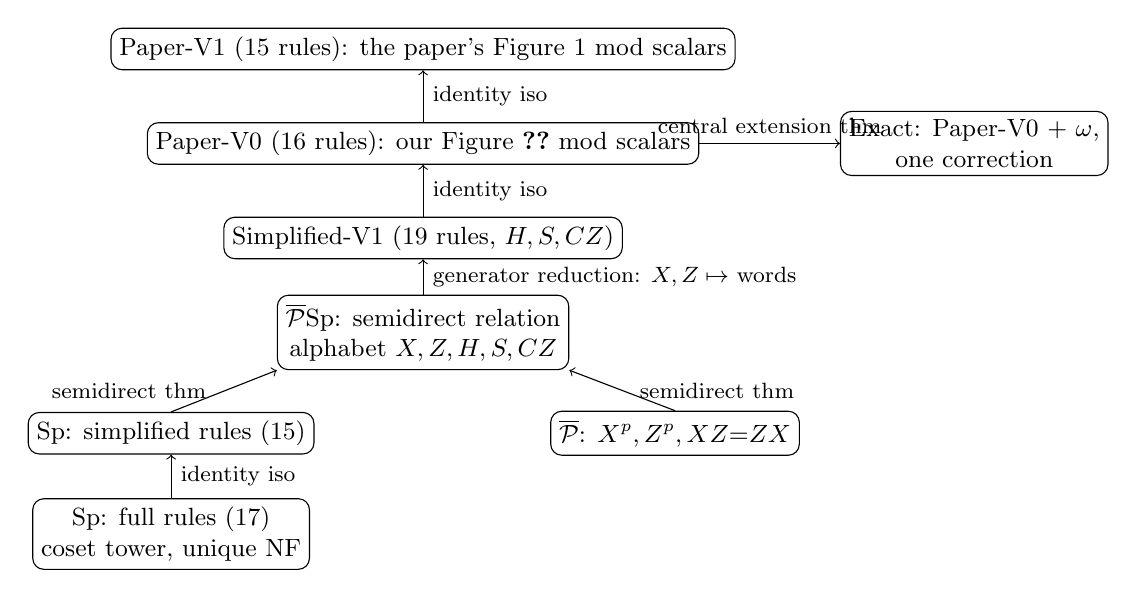
\begin{tikzpicture}[x=1cm,y=0.8cm,
  box/.style={draw,rounded corners,align=center,font=\small,inner sep=3pt},
  lab/.style={font=\footnotesize,align=center}]
  \node[box] (sp)  at (0,0)   {$\mathrm{Sp}$: full rules (17)\\ coset tower, unique NF};
  \node[box] (spsim) at (0,1.6) {$\mathrm{Sp}$: simplified rules (15)};
  \node[box] (pauli) at (6.4,1.6) {$\overline{\mathcal P}$: $X^p, Z^p, XZ{=}ZX$};
  \node[box] (sd)  at (3.2,3.2) {$\overline{\mathcal P}\rtimes\mathrm{Sp}$: semidirect relation\\ alphabet $X,Z,H,S,CZ$};
  \node[box] (v1)  at (3.2,4.7) {Simplified-V1 (19 rules, $H,S,CZ$)};
  \node[box] (v0)  at (3.2,6.2) {Paper-V0 (16 rules): our Figure~\ref{fig:rules} mod scalars};
  \node[box] (pv1) at (3.2,7.7) {Paper-V1 (15 rules): the paper's Figure~1 mod scalars};
  \node[box] (ex)  at (10.2,6.2) {Exact: Paper-V0 $+\ \omega$,\\ one correction};
  \draw[->] (sp) -- node[lab,right]{identity iso} (spsim);
  \draw[->] (spsim.north) -- node[lab,left,pos=0.5]{semidirect thm\ } (sd.south west);
  \draw[->] (pauli.north) -- node[lab,right,pos=0.5]{\ semidirect thm} (sd.south east);
  \draw[->] (sd) -- node[lab,right]{generator reduction: $X,Z\mapsto$ words} (v1);
  \draw[->] (v1) -- node[lab,right]{identity iso} (v0);
  \draw[->] (v0) -- node[lab,right]{identity iso} (pv1);
  \draw[->] (v0) -- node[lab,above]{central extension thm} (ex);
\end{tikzpicture}
\caption{The chain of presentations.  Every arrow is a verified
presentation theorem or a verified isomorphism of presentations; the
semantic group is $\mathrm{Sp}(2n,\mathbb Z_p)$ at the bottom,
$\overline{\mathcal P}_n \rtimes \mathrm{Sp}(2n,\mathbb Z_p)$ from the
semidirect level up, and a central extension of it by
$\langle\omega\rangle$ at the top right.}
\label{fig:route}
\end{figure}

Does this just move the difficulty around?  No.  The symplectic factor
is where the real rewriting happens, and keeping the Pauli part out of
it pays off everywhere: every box relation is an honest equation, every
coset-table entry is a function, and the Pauli bookkeeping that the
paper's Proposition~4.9 performs by hand is performed once, by the
semidirect-product theorem, in a form that was proved for arbitrary
groups before this project began.  The factored route is, we think, the
right way to organise such proofs even on paper.
